%%%%%%%%%%%%%%%%%%%%%%%%%%%%%%%%%%%%%%%%%%%%%%%%%%%%%%%%%%%%
% Document settings
\documentclass{ACGSeminar}

\bibliography{references}

%%%%%%%%%%%%%%%%%%%%%%%%%%%%%
% Hyphenations here
%%%%%%%%%%%%%%%%%%%%%%%%%%%%%
\hyphenation{}

%%%%%%%%%%%%%%%%%%%%%%%%%%%%%
% Title, Author, etc.

\begin{document}

\title{Efficient Ray Tracing Techniques}

\author{Dario Seyb}

\maketitle

%%%%%%%%%%%%%%%%%%%%%%%%%%%%%%%%%%%%%%%%%%%%%%%%%%%%%%%%%%%%
% Abstract

\begin{abstract}%
Ray Tracing is next to rasterization the most widely used technique to generate discrete 2D images from continuous 3D scenes. Until recently ray tracing was too resource intensive to produce images in realtime, but advances in hardware capabilities, most notably the introduction of GPGPU (General Purpose Graphics Processing Units), and algorithms made near-realtime ray tracing feasible. In this report we will present some of the techniques which are used to achieve this.
\end{abstract}

\keywords{Ray Tracing, Acceleration Structures, Realtime Rendering, GPGPU}
\tableofcontents

%%%%%%%%%%%%%%%%%%%%%%%%%%%%%%%%%%%%%%%%%%%%%%%%%%%%%%%%%%%%
% Introduction

\section{Introduction}

Talk about ray tracing from Whitted to Hyperion. 

%%%%%%%%%%%%%%%%%%%%%%%%%%%%%%%%%%%%%%%%%%%%%%%%%%%%%%%%%%%%
% Second Section
\section{Overview over the path tracing algorithm}
A short overview of the base algorithm we are going to use for the rest of the paper. Cite \cite{veach1997robust} all the way.

\section{Spacial partitioning and acceleration structures}
Going logarithmic!
\subsection{BSP and KD-Trees}
\subsection{Volume Hierarchies}

\section{Accelerating the convergence of path tracing}
Here's where \cite{Pharr:2010:PBR:1854996} comes in.
\subsection{Gradient-Domain Path Tracing}
Do I really want to go here? \cite{Kettunen2015sg} I'll implement everything else first and see if I have time left.
\subsection{Temporal Supersampling}
I need to find a real paper describing this, so far only GDC talks. I think this is going to make a huge difference in the quality I can achieve.

\section{Adapting the described algorithms to the GPU}
\subsection{Accessing the GPU outside of the rasterization pipeline}
CUDA or compute shaders, still need to decide.
\subsection{Hierarchical data structures on the GPU}
Use this: \cite{Karras:2012:MPC:2383795.2383801}

\section{Results}
I plan to implement everything I describe since I strongly believe computer science papers should \textbf{always} come with code.
\subsection{Images}
Pretty images rendered in real time. Link to a video.
\subsection{Timings}
Timing comparisons between the different techniques.


\begin{figure}[htb!]
  \begin{centering}
    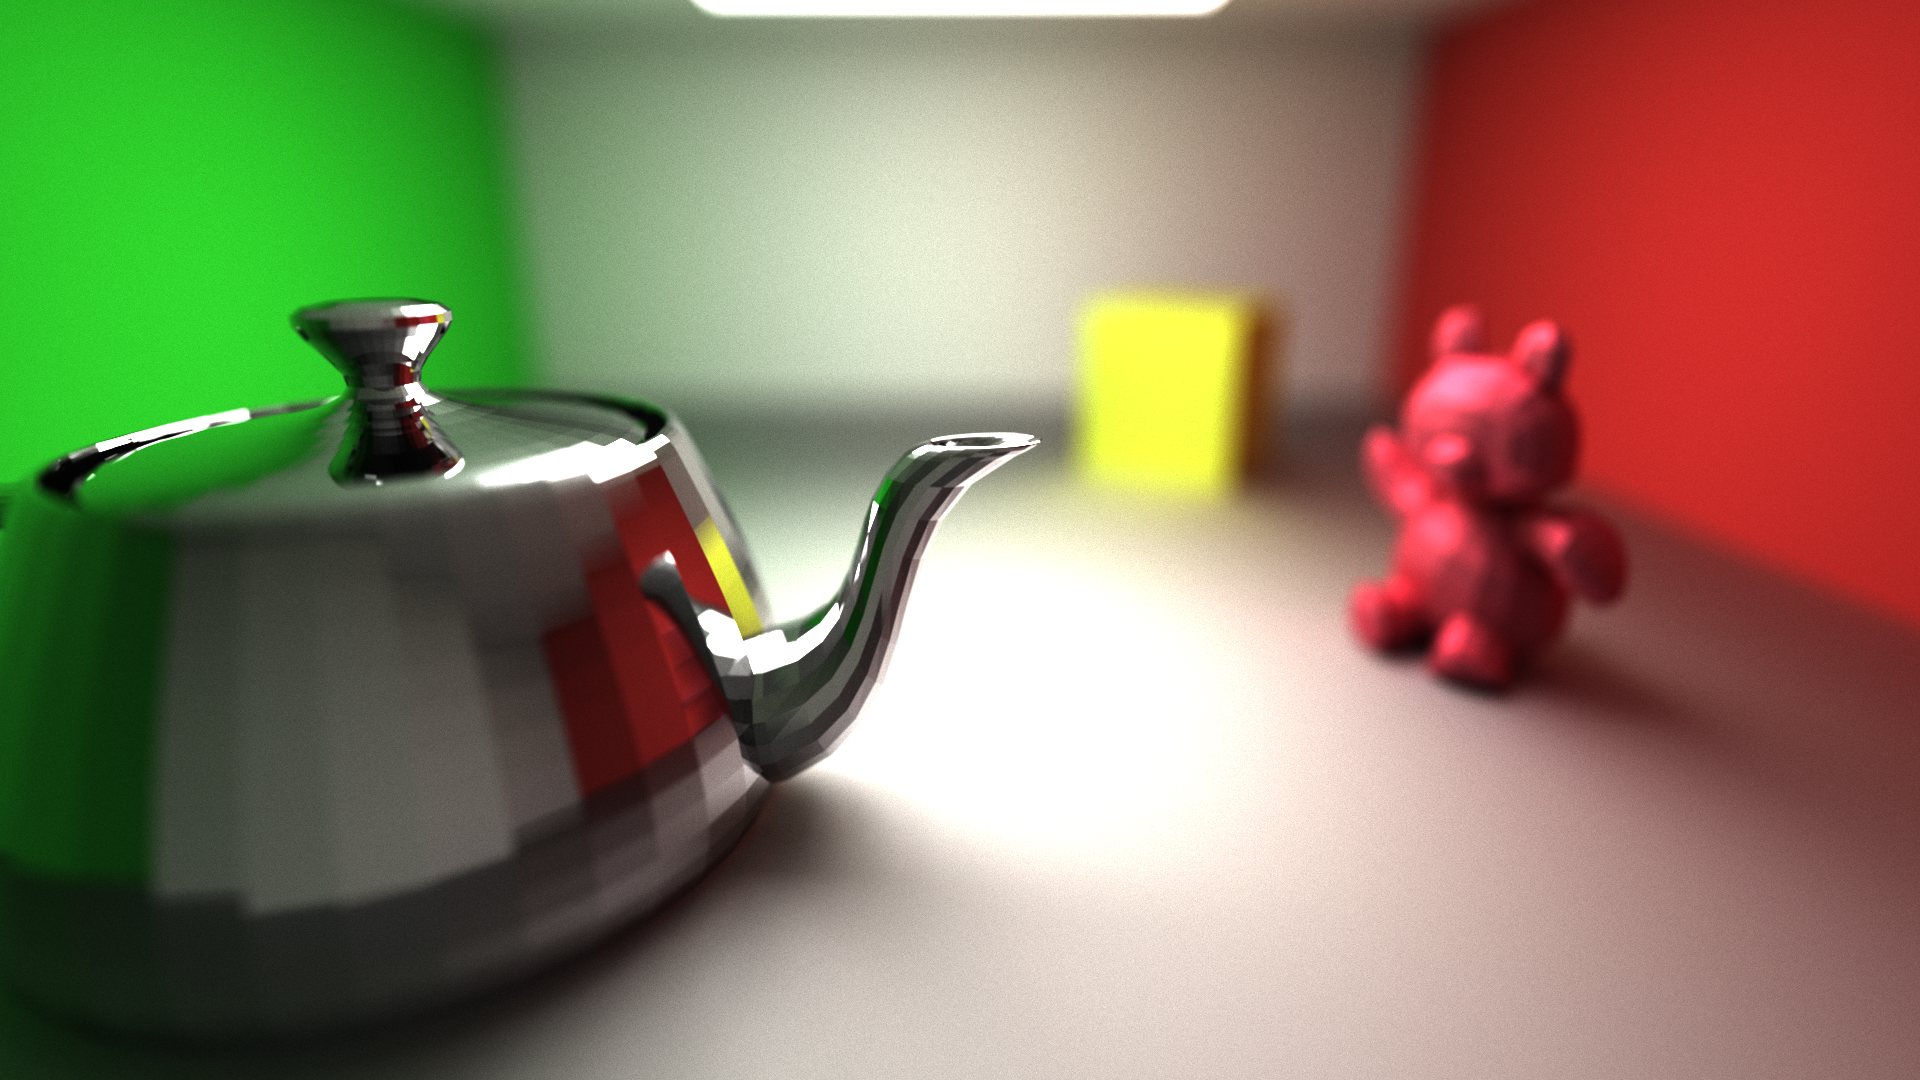
\includegraphics[width=10cm]{figures/Output_PT_10kSPP.png}\par
  \end{centering}
  \caption{This is what my path tracer is rendering right now, but not in real time.}
  \label{fig:pathtraced}
\end{figure}

%%%%%%%%%%%%%%%%%%%%%%%%%%%%%%%%%%%%%%%%%%%%%%%%%%%%%%%%%%%%
% Bibliography

\printbibliography
\cleardoublepage

\end{document}
